\section{System Design and Implementation}

\begin{figure}[!hb]   %% START_FIGURE
\centerline{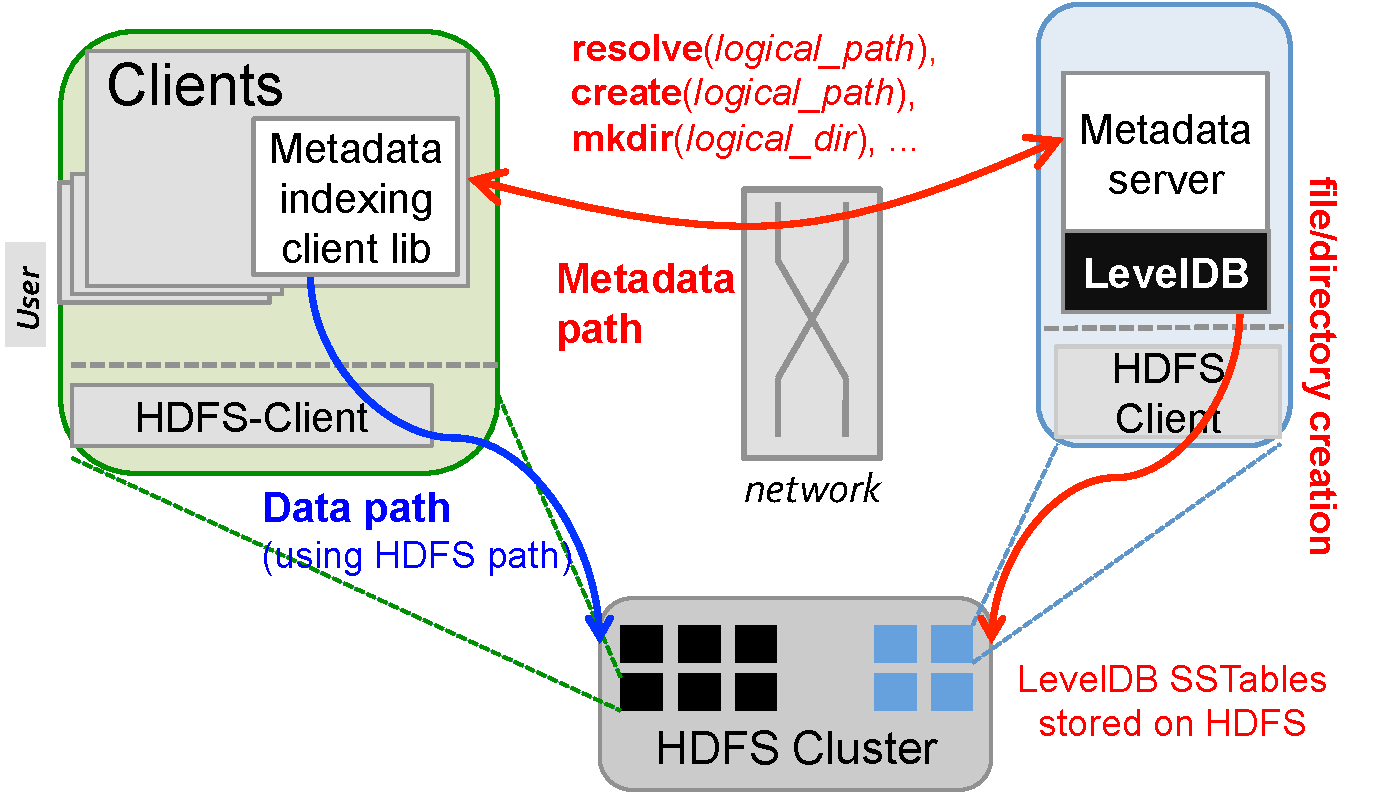
\includegraphics[scale=0.35]{./figs/giga-impl-leveldb-clusterfs}}
\vspace{10pt}
\caption{\textit{\footnotesize
The metadata servers deploys different policies to partition metadata
over multiple servers, and uses an Log-Structured Merge tree (LevelDB)
to manage out-of-core metadata representation on disk.
This integrated solution is layered on top of an existing distributed
file system deployment (e.g. HDFS) to improve its metadata and
small file operation efficiency.
}}
%\vspace{10pt}
\hrule
\label{fig:design}
\end{figure}       %% END_FIGURE

Figure \ref{fig:design} presents the overall architecture of our scalable
metadata service. Our metadata service is a middleware inserted into
existing deployments of distributed file systems to improve metadata efficiency
while maintaining high I/O bandwidth for data transfers.
The system uses a client-server architecture,
and consists of three core components:

\begin{itemize}
\item{\textbf{Client:}} Applications interact with our middleware
through a library directly linked into the application,
(or through the FUSE user-level file system \cite{fuse}).
The stateless client-side code redirects applications' file operations
to the appropriate destination according to the types of operations.
All metadata requests (e.g. \texttt{create()} and \texttt{mkdir()}),
and data requests on small files (e.g. \texttt{read()} and \texttt{write()}),
are handled by the metadata indexing modules that address
these requests to the appropriate server.
For all data operations on large size files, the client code redirects
the request directly to the underlying distributed file system to take full
advantage of data I/O bandwidth. A newly created, but growing file
may be transparently reopened by the client module.

\item{\textbf{Metadata Indexing Server:}}
Each indexing server manages its local metadata storage backend to store and
access all metadata information and small file data.
It can plug-in different indexing policies to
partition large directories across indexing servers.
It also monitors the growth of small files,
and migrates newly large files into the underlying distributed file system
when its size exceeds a threshold.

\item{\textbf{Metadata Storage Backend:}}
The metadata storage backend packs metadata and small file data into
large, log-structured, flat files, and stores these files
in the underlying distributed file system.
It uses a modified version of LevelDB \cite{leveldb} that
converts random updates into sequential writes, and improves disk performance.
In order to dynamically redistribute large directories,
the metadata storage backend also modifies LevelDB
to support exporting and importing a large list of key-value pairs in batch.

\end{itemize}

Remainder of this section describes more details of our system.
Section \ref{design.leveldb} shows how our metadata service
stores all file system metadata and small files
using a single on-disk structure on each server.
Section \ref{design.decouple} focus on the challenges in effectively
integrating our metadata middleware service with the underlying
distributed file systems. The rest sections discuss
distributed transaction support and fault tolerance strategy.

\subsection{Metadata Storage Backend}
\label{design.leveldb}

Our metadata storage backend implements a modified version of LevelDB
\cite{leveldb} to pack together and manage all the metadata and small files,
hiding them from the underlying cluster file system.
LevelDB is an open-source implementation of an Log-structure Merge (LSM) tree \cite{ONeil1996},
which provides a simple key-value store interface,
supporting point queries and range queries. In LevelDB, by default,
a set of changes are spilled to disk when the total size of modified
entries exceeds 4 MB.  When a spill is triggered,
the changed entries are sorted, indexed and written to disk
as an immutable file called an SSTable \cite{BigTable}.
These entries may then be discarded from the in memory buffer.
Discarded entries can be reloaded by searching each SSTable on disk,
possibly stopping when the first match occurs if the SSTables are
searched most recent to oldest.  The number of SSTables that need to be
searched is reduced by maintaining the minimum and maximum key value
and a Bloom filter\cite{bloomfilter} on each,
but, with time, the cost of finding a record not in memory still increases.
Compaction is the process of combining multiple overlapping range SSTables
into a number of disjoint range SSTables by merge sort.
More details about LevelDB can be found in its website \cite{leveldb}.

~\\
\textbf{Metadata representation: }
LevelDB aggregates directory entries,
inode attributes and small files into one LSM tree
with an entry for each file and directory.
To translate the hierarchical structure of the file system namespace
into key-value pairs, the 224-bit key is chosen to consist of
the 64-bit i-node number of a entry's parent directory
and a 160-bit SHA-1 hash value of its filename string
(final component of its pathname) as shown below:

\begin{table}[!htc]
\center
\vspace{10pt}
\begin{tabular}{c|c}
key & \texttt{Parent directory ID, hash(Object name)} \\
\midrule
value & \texttt{Attributes,[Symbolic link|Data]} \\
\end{tabular}
\label{tab:keyschema}
\end{table}

The value of an entry contains the file's full name and i-node attributes,
such as i-node number, ownership, access mode, file size, timestamps (\textit{struct stat} in Linux).
For small files with size less than $T$ (defaulting to 4KB),
the value field also contains the file's data.
For large files, the file data field in a file row of the table
is replaced by a symbolic link that points to
the actual file object in the underlying file system.
LevelDB also preserve additional information for different
indexing policy. For dynamic namespace partition,
it also records hash partition related mapping information for directories
used in \giga.

~\\
\textbf{Partition splitting: }
To effectively build indexing server that integrates
the dynamic namespace distribution mechanism
and our on-disk metadata representation,
we have to modify LevelDB to support for
migrating directory partitions as required by \giga.

The file system metadata, including \giga directory partitions and their directory
entries are stored in \ldb as a set of immutable files (SSTable files)
in a server specific directory in the underlying distributed file system.
Each metadata indexing server process splits a large partition $P$ on
into itself and another hash partition $P'$ which is managed by a
different server; this split involves migrating approximately half the entries
from old partition $P$ to the new partition $P'$ on another server.
During splitting, the partition in migration is locked against client
for simplification. We explored several ways
to perform this cross-server partition split.

A straightforward solution would be to perform a range scan on
partition $P$, and remove about half the entries
(that will be migrated to the new partition $P'$) from $P$.
All removed entries would then be batched together
and sent in a large RPC message to the server that will manage partition $P'$.
The split receiver would insert each key in the batch into its own \ldb instance.
While simplicity of this solution makes it attractive,
it is slow in practice and vulnerable to failures during splitting.

We have devised a faster and safer technique to
reduce the time that the splitting range is locked.
The immutability of SSTables in \ldb makes a fast bulk insert possible --
an SSTable whose range does not overlap any part of a current LSM tree
can be added to Level 0 without its data being pushed through the
write-ahead log and minor compaction process.
To take advantage of this opportunity, we extended \ldb
to support a three-phase \giga split operation:

\begin{itemize}
\item{Phase 1:} The split initiator locks and
then performs a range scan on its \ldb instance
to find all entries in the hash-range that needs to be moved to another server.
Instead of packing these into an RPC message,
the results of this scan are written in SSTable format to a file in the
underlying distributed file system.

\item{Phase 2:} The split initiator notifies the split receiver about
the path to the SSTable-format split file in a much smaller RPC message.
Since this file is stored in shared storage,
the split receiver directly inserts this file as a symbolic link
into the \ldb tree structure without actually copying this file.
The insertion of this file into the split receiver is the commit
part of the split transaction.

\item{Phase 3:} The final step is a clean-up phase:
after the split receiver completes the bulk insert operation, it notifies the
initiator, who then deletes the migrated key-range from its \ldb instance
and unlocks the range.
\end{itemize}


\subsection{Decoupled Data and Metadata Path}
\label{design.decouple}

\subsection{Transaction Support}

\subsection{Fault Tolerance}

